%https://latexdraw.com/draw-flowcharts-latex-tutorial/

%https://tex.stackexchange.com/questions/8890/tikz-how-to-draw-boxes-around-set-of-nodes

%https://tikz.dev/tikz-shapes

%https://tex.stackexchange.com/questions/8890/tikz-how-to-draw-boxes-around-set-of-nodes

%https://www.latex4technics.com/?note=189T

\documentclass[border=0.2cm]{standalone}
 
% Required packages
\usepackage{comment}
\usepackage{tikz}
\usetikzlibrary{shapes,positioning,calc}


\usepackage{color}
\definecolor{franklinblue}{RGB}{0,43,83}
\definecolor{cardinalred}{RGB}{140,21,21}
\definecolor{skobeloff}{rgb}{0.0, 0.48, 0.45}
\definecolor{auburn}{rgb}{0.43, 0.21, 0.1}
\definecolor{calpolypomonagreen}{rgb}{0.12, 0.3, 0.17}
\definecolor{ao(english)}{rgb}{0.0, 0.5, 0.0}

\tikzset{
    ncbar angle/.initial=90,
    ncbar/.style={
        to path=(\tikztostart)
        -- ($(\tikztostart)!#1!\pgfkeysvalueof{/tikz/ncbar angle}:(\tikztotarget)$)
        -- ($(\tikztotarget)!($(\tikztostart)!#1!\pgfkeysvalueof{/tikz/ncbar angle}:(\tikztotarget)$)!\pgfkeysvalueof{/tikz/ncbar angle}:(\tikztostart)$)
        -- (\tikztotarget)
    },
    ncbar/.default=0.5cm,
}
\tikzset{square left brace/.style={ncbar=0.5cm}}
\tikzset{square right brace/.style={ncbar=-0.5cm}}
 
\begin{document}
 
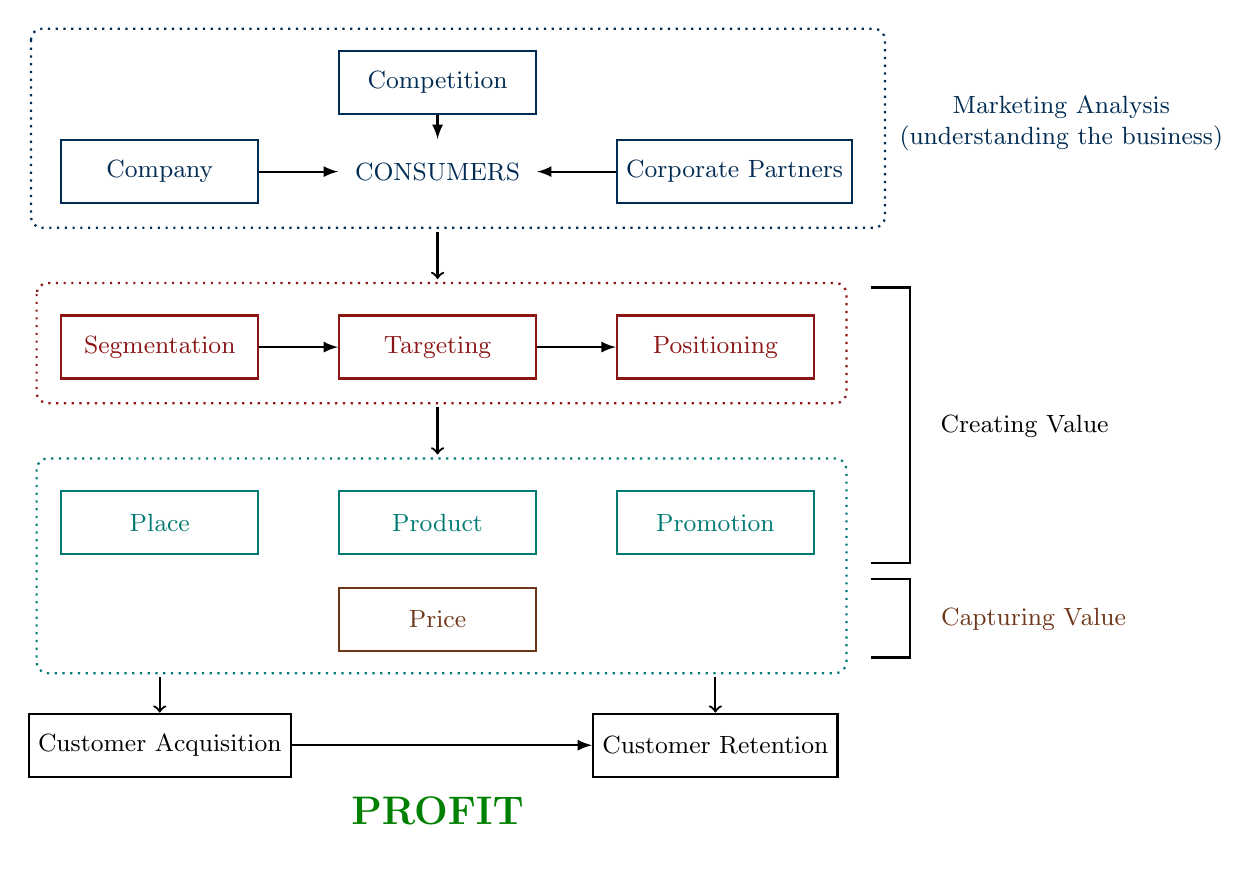
\begin{tikzpicture}[font=\small,thick,align=center]
 
% Start block - Competition node
\node[draw=franklinblue,
    text=franklinblue,
    rectangle,
    minimum width=2.5cm,
    minimum height=0.8cm] (block1) {Competition};

% Consumer node
\node[%draw=franklinblue,
    text=franklinblue,
    %rectangle,
    below=of block1,
    yshift=0.7cm,
    minimum width=2.5cm,
    minimum height=0.8cm] (block2) {CONSUMERS};
 
% Company node
\node[draw=franklinblue,
    text=franklinblue,
    rectangle,
    left=of block2,
    minimum width=2.5cm,
    minimum height=0.8cm] (block3) {Company};

% Corporate Partners node
\node[draw=franklinblue,
    text=franklinblue,
    rectangle,
    right=of block2,
    minimum width=2.5cm,
    minimum height=0.8cm] (block4) {Corporate Partners};

% Targeting
\node[draw=cardinalred,
    text=cardinalred,
    rectangle,
    below=of block2,
    yshift=-0.4cm,
    minimum width=2.5cm,
    minimum height=0.8cm] (block5) {Targeting};

% Segment
\node[draw=cardinalred,
    text=cardinalred,
    rectangle,
    left=of block5,
    minimum width=2.5cm,
    minimum height=0.8cm] (block6) {Segmentation};

% Positioning
\node[draw=cardinalred,
    text=cardinalred,
    rectangle,
    right=of block5,
    minimum width=2.5cm,
    minimum height=0.8cm] (block7) {Positioning}; 

% Product
\node[draw=skobeloff,
    text=skobeloff,
    rectangle,
    below=of block5,
    yshift=-0.4cm,
    minimum width=2.5cm,
    minimum height=0.8cm] (block8) {Product};

% Place
\node[draw=skobeloff,
    text=skobeloff,
    rectangle,
    left=of block8,
    minimum width=2.5cm,
    minimum height=0.8cm] (block9) {Place};

% Promotion
\node[draw=skobeloff,
    text=skobeloff,
    rectangle,
    right=of block8,
    minimum width=2.5cm,
    minimum height=0.8cm] (block10) {Promotion};    

% Price
\node[draw=auburn,
    text=auburn,
    rectangle,
    below=of block8,
    yshift=0.6cm,
    minimum width=2.5cm,
    minimum height=0.8cm] (block11) {Price};

% Customer Acquisition
\node[draw=black,
    text=black,
    rectangle,
    below=of block9,
    yshift=-1.0cm,
    %xshift=1.0cm,
    minimum width=2.5cm,
    minimum height=0.8cm] (block12) {Customer Acquisition};

% Customer Retention
\node[draw=black,
    text=black,
    rectangle,
    below=of block10,
    yshift=-1.0cm,
    %xshift=1.0cm,
    minimum width=2.5cm,
    minimum height=0.8cm] (block13) {Customer Retention}; 

% Profit
\node[%draw=auburn,
    text=ao(english),
    %rectangle,
    below=of block11,
    yshift=-0.6cm,
    minimum width=2.5cm,
    minimum height=0.8cm] (block14) {{\Large \textbf{PROFIT}}};  

%Commentary Boxes
% First Box Commentary
\node[%draw=franklinblue,
    text=franklinblue,
    %rectangle,
    right=of block1,
    minimum width=2.5cm,
    minimum height=0.8cm] (blockA)  [below right=-1.5cm and 8cm of block3]
    {Marketing Analysis \\ (understanding the business)};

% Second Box Commentary
\node[%draw=franklinblue,
    text=black,
    %rectangle,
    right=of block7,
    xshift=0.4cm,
    yshift=-1.0cm,
    minimum width=2.5cm,
    minimum height=0.8cm] (blockB) 
    {Creating Value};

% Third Box Commentary
\node[%draw=franklinblue,
    text=auburn,
    %rectangle,
    right=of block11,
    xshift=4.0cm,
    minimum width=2.5cm,
    minimum height=0.8cm] (blockC) 
    {Capturing Value};

% Arrows
\draw[-latex] (block1) edge (block2)
    (block3) edge (block2)
    (block4) edge (block2);

\draw[-latex] (block6) edge (block5)
    (block5) edge (block7);

\draw[-latex] (block12) edge (block13);

\draw[shorten >= 0.45cm, shorten <= 0.35cm, ->] (block2) edge (block5);    

\draw[shorten >= 0.45cm, shorten <= 0.35cm, ->] (block5) edge (block8);   

\draw[shorten >= 0.0cm, shorten <= 1.55cm, ->] (block9) edge (block12);   

\draw[shorten >= 0.0cm, shorten <= 1.55cm, ->] (block10) edge (block13); 


% Boxes around Nodes
\draw[franklinblue,thick,dotted, rounded corners] ($(block2.north west)+(-3.9,1.4)$)  rectangle ($(block4.south east)+(0.4,-0.3)$);

\draw[cardinalred,thick,dotted, rounded corners] ($(block6.north west)+(-0.3,0.4)$)  rectangle ($(block7.south east)+(0.4,-0.3)$);

\draw[skobeloff,thick,dotted, rounded corners] ($(block9.north west)+(-0.3,0.4)$)  rectangle ($(block10.south east)+(0.4,-1.5)$);

%Braces
\draw[black, thick] (5.5,-2.6) to [square left brace ] (5.5,-6.1);
\draw[black, thick] (5.5,-6.3) to [square left brace ] (5.5,-7.3);

%%%%%%%%%%%%%%%%%%%%%%%

% Power and voltage variation
\begin{comment}
\node[draw,
    below=of block2,
    minimum width=3.5cm,
    minimum height=1cm
] (block3) { $\Delta P=P_k-P_{k-1}$ \\ $\Delta V=V_k-V_{k-1}$};


% Conditions test
\begin{comment}
\node[draw,
    diamond,
    below=of block3,
    minimum width=2.5cm,
    inner sep=0] (block4) { $\Delta P>0$};

\node[draw,
    diamond,
    below left=of block4,
    minimum width=2.5cm,
    inner sep=0] (block5) { $\Delta V>0$};
 
\node[draw,
    diamond,
    below right=of block4,
    minimum width=2.5cm,
    inner sep=0] (block6) { $\Delta V>0$};
 
% Increase and Decrease duty cycle
\node[draw,
    below=of block5,
    minimum width=2.5cm,
    minimum height=1cm] (block7) { $D=D+\Delta D$};
 
\node[draw,
    left=of block7,
    minimum width=2.5cm,
    minimum height=1cm] (block8) { $D=D-\Delta D$};
 
\node[draw,
    below=of block6,
    minimum width=2.5cm,
    minimum height=1cm] (block9) { $D=D-\Delta D$};
 
\node[draw,
    right=of block9,
    minimum width=2.5cm,
    minimum height=1cm] (block10) { $D=D+\Delta D$};
 
% Return block
\node[draw,
    rounded rectangle,
    below=5cm of block4,
    minimum width=2.5cm,
    minimum height=1cm,] (block11) { RETURN};
 
\node[coordinate,below=4.35cm of block4] (block12) {};
 
 
% Arrows
\draw[-latex] (block1) edge (block2)
    (block3) edge (block2)
    (block4) edge (block2);
 

\begin{comment}
\draw[-latex] (block4) -| (block5)
    node[pos=0.25,fill=white,inner sep=0]{Yes};
 
\draw[-latex] (block4) -| (block6)
    node[pos=0.25,fill=white,inner sep=0]{No};
 

\draw[-latex] (block5) edge node[pos=0.4,fill=white,inner sep=2pt]{No}(block7)
    (block5) -| (block8)
        node[pos=0.25,fill=white,inner sep=0]{Yes};
 
\draw[-latex] (block6) edge node[pos=0.4,fill=white,inner sep=2pt]{No}(block9)
    (block6) -| (block10)
        node[pos=0.25,fill=white,inner sep=0]{Yes};
 
\draw (block7) |- (block12);
\draw (block9) |- (block12);
\draw (block8) |- (block7|-block12);
\draw (block10) |- (block9|-block12);
\draw[-latex] (block12) -- (block11);
 
\end{comment} 

\end{tikzpicture}
 
\end{document}